\chapter{Implementacija i korisničko sučelje}


\section{Korištene tehnologije i alati}


\hspace{0.67cm}Komunikacija u timu odvijala se putem aplikacija \underline{WhatsApp}\footnote{\url{https://www.whatsapp.com/}} i \underline{Discord}\footnote{\url{https://discord.com/}}.
Kao sustav za upravljanje izvornim kodom korišten je \underline{Git}\footnote{\url{https://git-scm.com/}}, distribuirani sustav kontrole verzija koji prati promjene u bilo kojem skupu datoteka. Udaljeni repozitorij projekta je dostupan na web platformi \underline{GitLab}\footnote{\url{https://about.gitlab.com/}}.

UML dijagrami su napravljeni u \underline{Visual Paradigm Online}\footnote{\url{https://www.visual-paradigm.com/}}, besplatnom alatu za crtanje.

Pri oblikovanju aplikacije za \textit{backend}  je korišten radni okvir \underline{Spring Boot}\footnote{\url{https://spring.io/projects/spring-boot/}} i jezik \underline{Java}\footnote{\url{https://www.java.com/en/}}. Spring Boot je otvoreni Java radni okvir namijenjen pojednostavljenoj izgradnji samostalnih, produkcijski orijentiranih Spring aplikacija. Pruža optimiziranu platformu za razvoj Java aplikacija s naglaskom na konvenciju umjesto konfiguracije, omogućavajući programerima brzo postavljanje i razvoj robusnih, skalabilnih i efikasnih aplikacija. Spring Boot dolazi s ugrađenim značajkama poput automatske konfiguracije, podrške za ugrađeni web poslužitelj i postavkama spremnim za produkcijsko okruženje. Java je objektno orijentirani i platformski neovisan programski jezik. Kod napisan u Javi može izvoditi na bilo kojem uređaju ili platformi s Java Virtual Machine (JVM). Java je poznata po svojoj prenosivosti, snažnoj podršci zajednice i obilnim bibliotekama, što je čini popularnim izborom za izgradnju različitih vrsta aplikacija.




Za implementaciju \textit{frontenda} koristili smo razvojno okruženje \underline{React}\footnote{\url{https://react.dev/}} i jezik \underline{JavaScript}\footnote{\url{https://www.javascript.com/}}. React je otvorena JavaScript biblioteka za izgradnju korisničkih sučelja. Omogućuje stvaranje ponovno upotrebljivih komponenti korisničkog sučelja, upravljanje njihovim vlastitim stanjem i učinkovito ažuriranje korisničkog sučelja putem virtualnog DOM-a. React slijedi jednosmjerni tok podataka, koristi JSX za sintaksu komponenata i široko se koristi zbog modularnosti i optimizacija performansi.
JavaScript je svestrani i objektno orijentirani jezik, uglavnom korišten za stvaranje dinamičnog i interaktivnog sadržaja na web stranicama. Podržava asinkrono programiranje i radi na različitim platformama, što ga čini ključnom tehnologijom u web razvoju. Osim u preglednicima, proširuje se i na druge domene, uključujući i izradu mobilnih aplikacija. 

\underline{LaTeX}\footnote{\url{https://www.latex-project.org/}} je sustav za stvaranje visokokvalitetnih dokumenata, posebno u znanstvenim i akademskim kontekstima. Koristi označavanje teksta pomoću naredbi kako bi se definirala struktura dokumenta i formatiranje. Korisnici pišu dokumente u običnom tekstu s ekstenzijom .tex i koriste LaTeX compiler za generiranje formatiranih izlaza, često u PDF formatu.


\eject 


\section{Ispitivanje programskog rješenja}




\subsection{Ispitivanje komponenti}

Ispitivanje komponenti provjerava ispravnost djelovanja pojedinih dijelova programa koji su mogući za odvojeno ispitivanje, poput pojedinačnih funkcija ili metoda unutar objekta. U ovom projektu koristimo JUnit i Mockito za implementaciju i izvođenje automatskih testova. JUnit je okvir za testiranje koji omogućuje definiranje, organiziranje i izvođenje testova kako bismo provjerili ispravnost funkcionalnosti naše aplikacije. Mockito je biblioteka koja nam omogućuje stvaranje lažnih objekata kako bismo simulirati njihovu funkcionalnost, omogućujući izolaciju jedinica koda i neovisno testiranje. Pomoću Mockito-a smo stvorili mock objekte za servise i repozitorije, što nam omogućuje precizno kontroliranje ponašanja tih objekata tijekom testiranja.

\begin{figure}[H]
	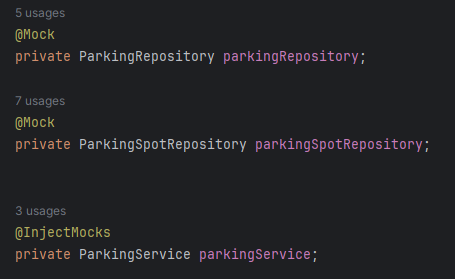
\includegraphics[width=\textwidth]{slike/mock.png} %veličina slike u odnosu na originalnu datoteku i pozicija slike
	\centering
	\caption{Stvaranje mock objekata}
	\label{fig:dijagramstanja}
\end{figure}



Ispitivanje komponenti za CreateKorisnikTest fokusira se na verifikaciju funkcionalnosti klase KorisnikService prilikom stvaranja novog korisnika. Testiraju se različiti scenariji, uključujući prepoznavanje već postojećeg emaila ili korisničkog imena te obrada null vrijednosti slike.

\begin{figure}[H]
	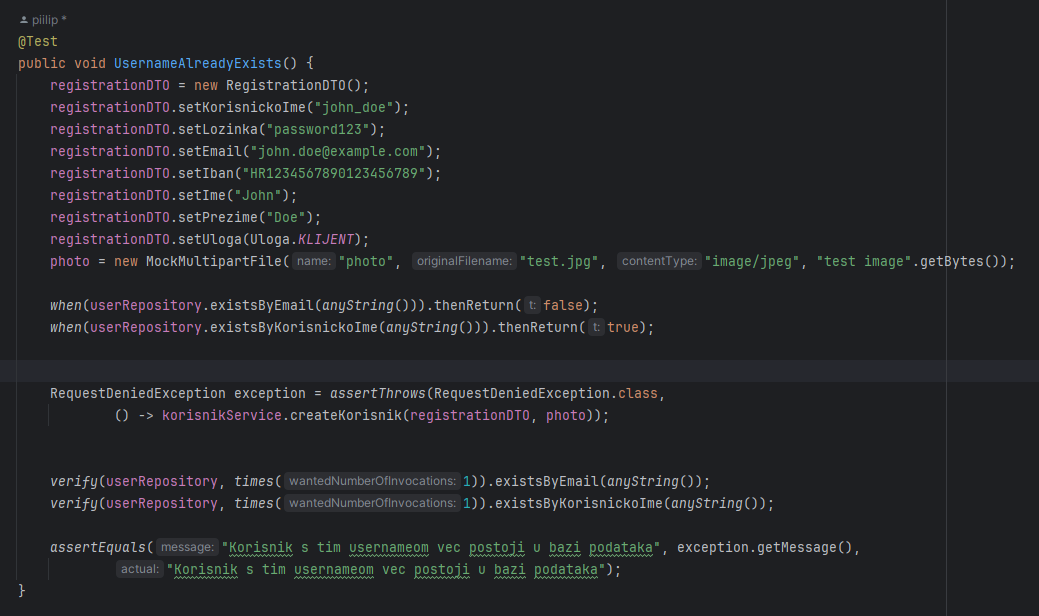
\includegraphics[width=\textwidth]{slike/username.png} %veličina slike u odnosu na originalnu datoteku i pozicija slike
	\centering
	\caption{1. ispitni slučaj za CreateKorisnikTest}
	\label{fig:dijagramstanja}
\end{figure}

\begin{figure}[H]
	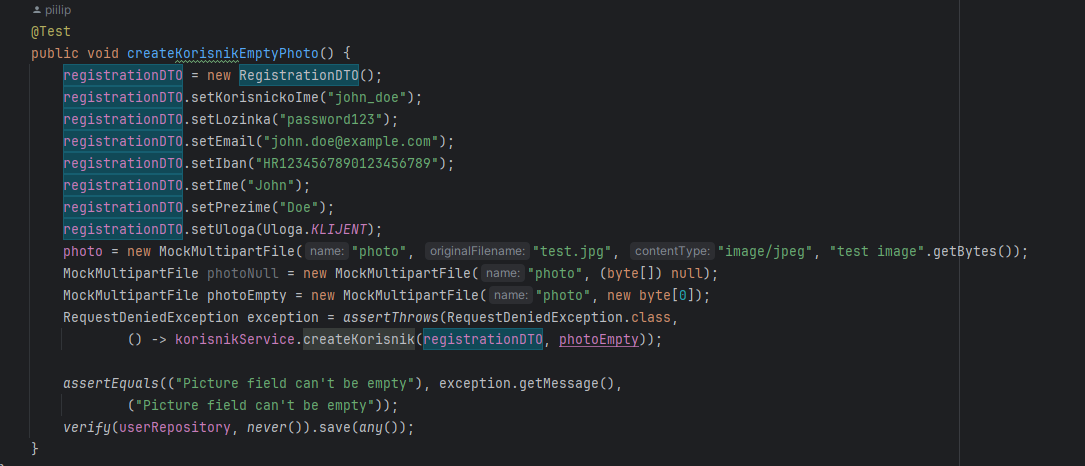
\includegraphics[width=\textwidth]{slike/korisnikslika.png} %veličina slike u odnosu na originalnu datoteku i pozicija slike
	\centering
	\caption{2. ispitni slučaj za CreateKorisnikTest}
	\label{fig:dijagramstanja}
\end{figure}

\begin{figure}[H]
	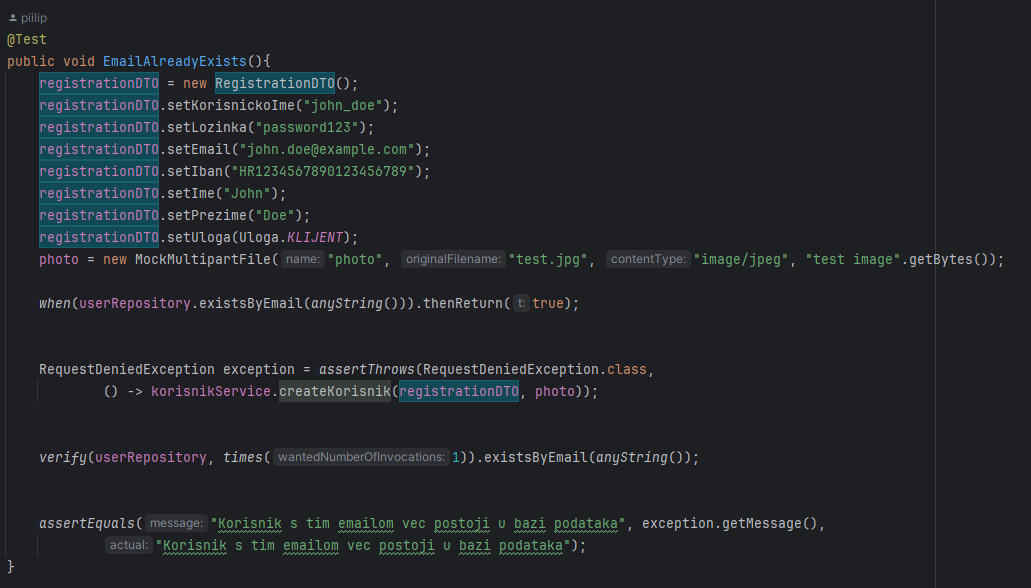
\includegraphics[width=\textwidth]{slike/email.png} %veličina slike u odnosu na originalnu datoteku i pozicija slike
	\centering
	\caption{3. ispitni slučaj za CreateKorisnikTest}
	\label{fig:dijagramstanja}
\end{figure}

Ispitivanje komponenti za UpdateKorisnikTest usmjereno je na verifikaciju funkcionalnosti metode updateKorisnik unutar klase KorisnikService. Testiraju se scenariji ažuriranja korisničkih podataka, uključujući promjenu korisničkog imena, imena, lozinke i slike.

\begin{figure}[H]
	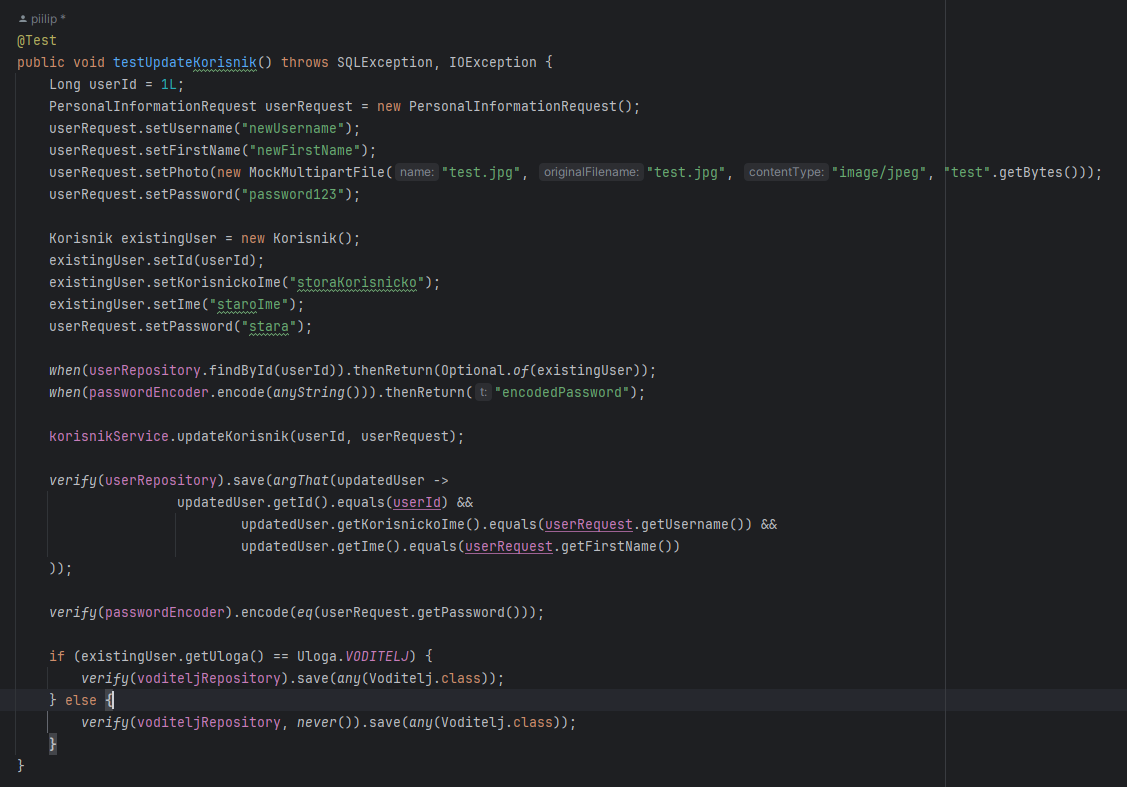
\includegraphics[width=\textwidth]{slike/testupdatekorisnik.png} %veličina slike u odnosu na originalnu datoteku i pozicija slike
	\centering
	\caption{1. ispitni slučaj za UpdateKorisnikTest}
	\label{fig:dijagramstanja}
\end{figure}


Ispitivanje komponenti za ParkingServiceTest usmjereno je na verifikaciju funkcionalnosti klase ParkingService. Fokusirano je na ispravno označavanje parkirnih mjesta kao rezervirana i ponašanje sustava u različitim scenarijima(verifikacija ispravnosti označavanja parkirnih mjesta kao rezervirana, provjera ponašanja sustava u slučaju nepostojećeg parkirališta, verifikacija ponašanja sustava kada je parkirno mjesto već označeno i testiranje ispravnosti dobivanja indeksa najmanje udaljenosti). Provjeravamo metodu markSpots koja je dio ParkingServicea. 
Ta metoda će pridružiti dana parkirališna mjesta s parkiralištem, osim u slučaju kad parkirno već pripada nekom drugom parkiralištu. U slučaju kad su sva mjesta uspješno rezervirana ta metoda vraća null vrijednost, a u suprotnom vraća listu onih mjesta koja nismo uspjeli rezervirati.
U testu markSpotsSuccess metode želimo provjeriti hoće li metoda vratiti null vrijednost, ako smo rezervirali sva mjesta. Testiramo samo s jednim parkingSpotom koje nema označen Parking, odnosno parkingSpot.getParking() == null i zbog toga očekujemo da će povratna vrijednost poziva markSpots biti null. 

\begin{figure}[H]
	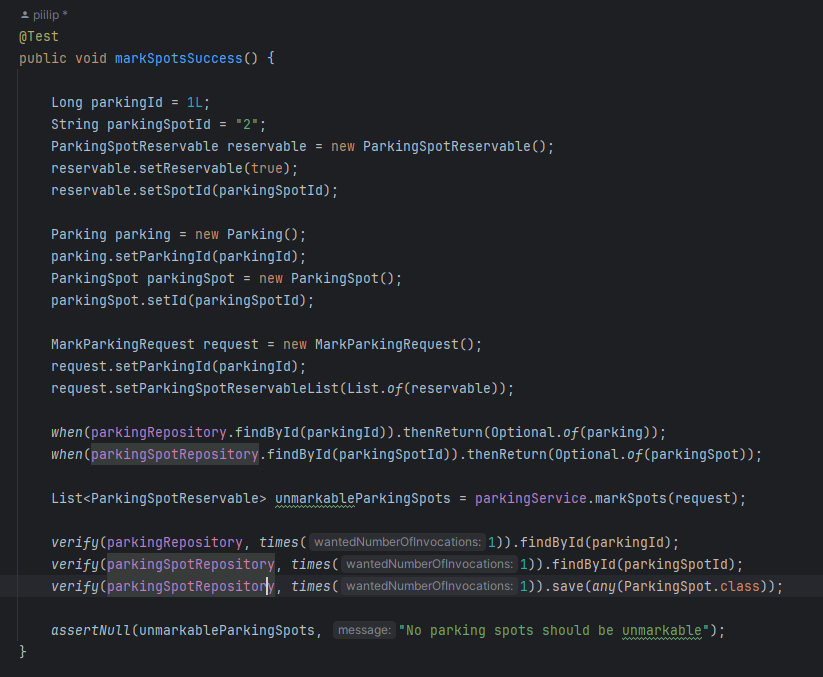
\includegraphics[width=\textwidth]{slike/markspotsuccess.png} %veličina slike u odnosu na originalnu datoteku i pozicija slike
	\centering
	\caption{1. ispitni slučaj za ParkingServiceTest}
	\label{fig:dijagramstanja}
\end{figure}


S testom markSpotsSomeFoundSomeNot testiramo slučaj kad imamo jedno ispravno i jedno neispravno mjesto. Odnosno kad imamo jedno mjesto koje već pripada nekom parkiralištu i jedno koje ne pripada. U tom slučaju bi trebali spremiti ispravno parkiralište (broj poziva parkingSpotRepository.save() bi trebao biti jedan) i vratiti neispravna mjesta.


\begin{figure}[H]
	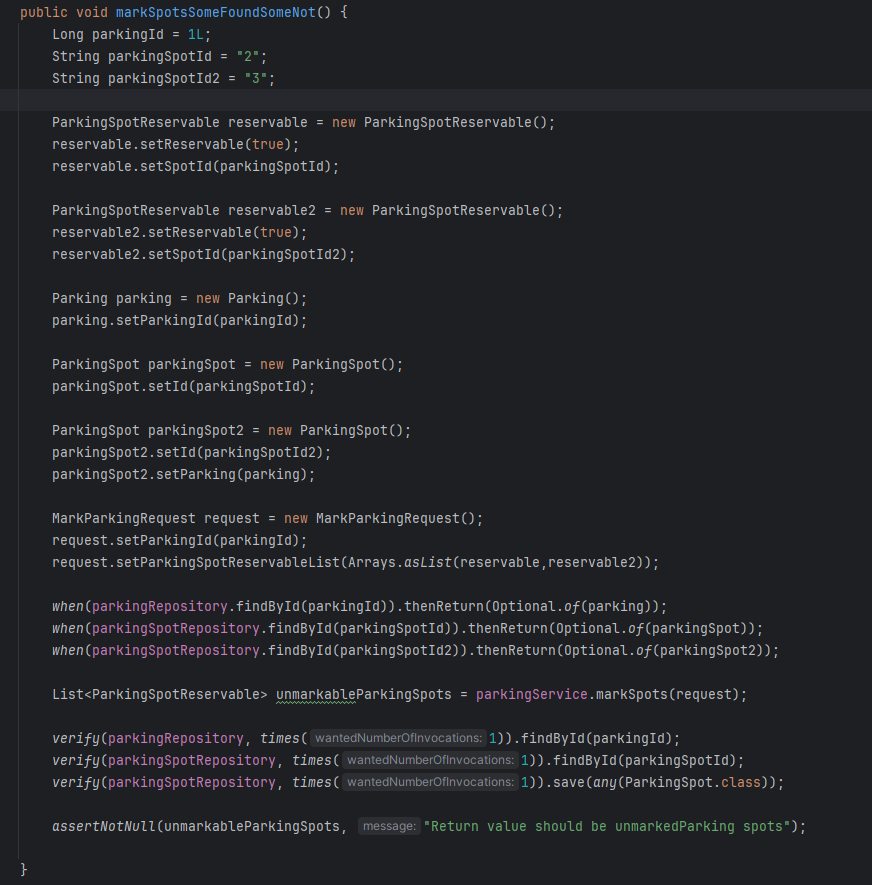
\includegraphics[width=\textwidth]{slike/markspotfound.png} %veličina slike u odnosu na originalnu datoteku i pozicija slike
	\centering
	\caption{2. ispitni slučaj za ParkingServiceTest}
	\label{fig:dijagramstanja}
\end{figure}

\begin{figure}[H]
	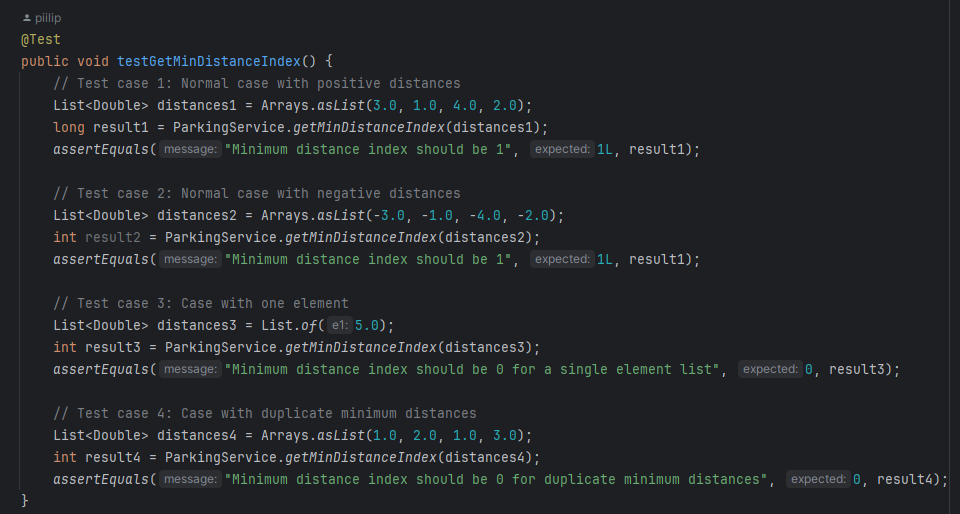
\includegraphics[width=\textwidth]{slike/testmindistance.png} %veličina slike u odnosu na originalnu datoteku i pozicija slike
	\centering
	\caption{3. ispitni slučaj za ParkingServiceTest}
	\label{fig:dijagramstanja}
\end{figure}

\begin{figure}[H]
	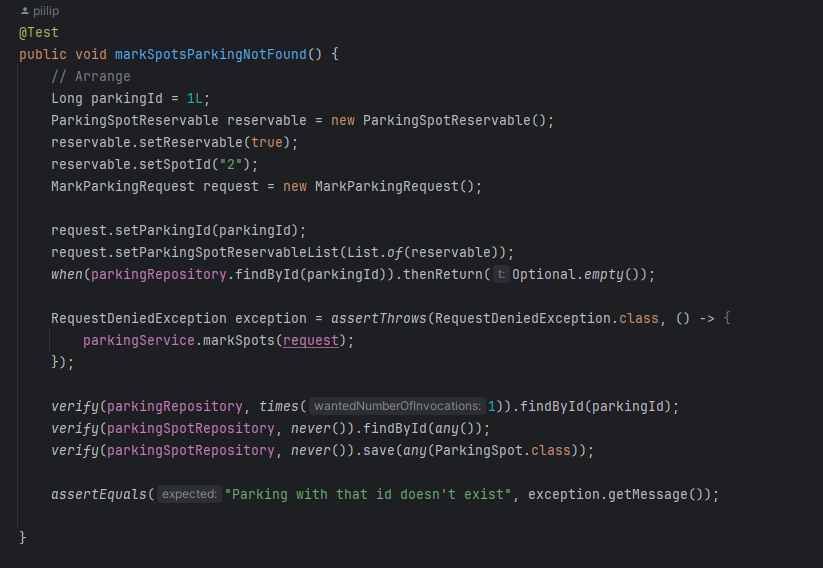
\includegraphics[width=\textwidth]{slike/markspotparking.png} %veličina slike u odnosu na originalnu datoteku i pozicija slike
	\centering
	\caption{4. ispitni slučaj za ParkingServiceTest}
	\label{fig:dijagramstanja}
\end{figure}


\begin{figure}[H]
	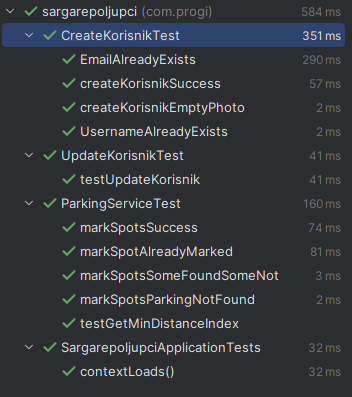
\includegraphics[width=\textwidth]{slike/results.png} %veličina slike u odnosu na originalnu datoteku i pozicija slike
	\centering
	\caption{Rezultati svih ispitnih slučajeva}
	\label{fig:dijagramstanja}
\end{figure}

\subsection{Ispitivanje sustava}

\eject 


\section{Dijagram razmještaja}


UML-dijagrami razmještaja (engl. deployment diagrams) su takoder vrsta strukturnih UML-dijagrama koji prikazuju fizičku arhitekturu i konfiguraciju razmještaja programskog sustava. Oni ilustriraju raspodjelu programskih komponenti, izvršnih datoteka i knjižnica na sklopovske čvorove ili virtualna izvršna okruženja.
Na poslužiteljskom računalu nalaze se Web poslužitelj i poslužitelj baze podataka. Korisnik do web aplikacije dolazi preko web preglednika pri čemu mobilna aplikacija komunicira s poslužiteljem pomoću protokola HTTP. Osim s korisnikom, web poslužitelj komunicira i s OSRM pomoću protokola HTTP.

\vspace{5cm}

\begin{figure}[H]
	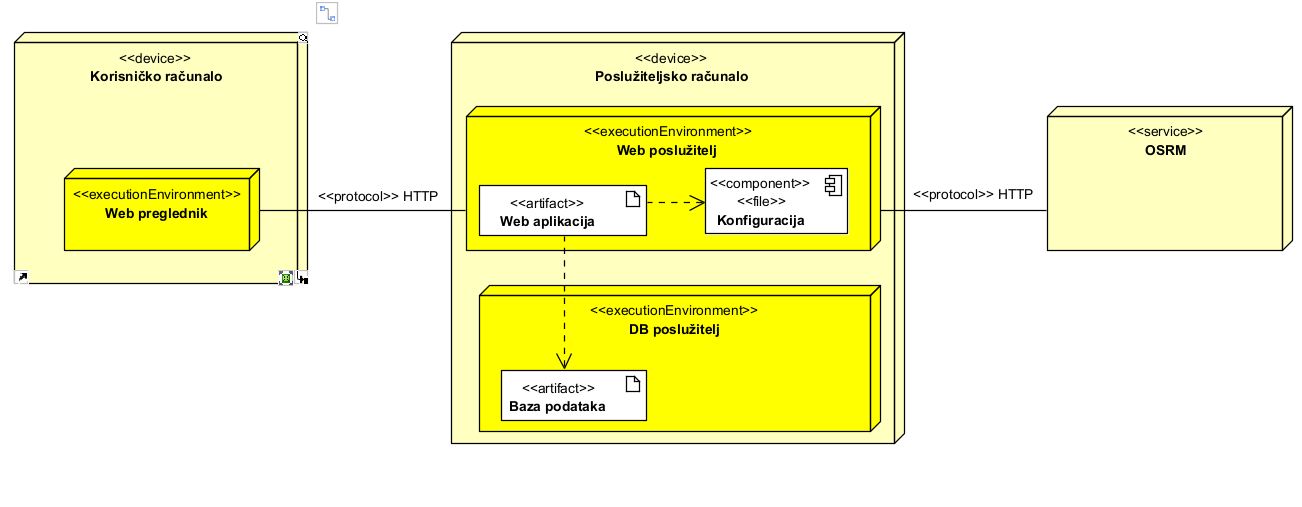
\includegraphics[width=\textwidth]{slike/dijagram_razmjestaja.png} %veličina slike u odnosu na originalnu datoteku i pozicija slike
	\centering
	\caption{Dijagram razmještaja}
	\label{fig:dijagramaktivnosti}
\end{figure}
\eject 

\section{Upute za puštanje u pogon}

Prvo, preuzmite glavnu granu repozitorija ove web aplikacije putem naredbe "git pull" s GitLab-a.

Za implementaciju na Renderu, preporučljivo je stvoriti račun na GitHub-u ili GitLab-u i povezati ga s Renderom. Nakon stvaranja računa, možete dodati web aplikaciju kao novi projekt na svom računu.

Što se tiče baze podataka na Renderu, prijavite se, kliknite na gumb "New" u gornjem desnom kutu i odaberite opciju "PostgreSQL". Unesite identifikacijske podatke i konfiguracijske informacije, poput lako prepoznatljivog imena baze (koje će se prikazivati u Renderu), stvarnog imena baze podataka, korisničkog imena i odabira regije. Ostavite verziju PostgreSQL-a na zadanim postavkama, osim ako imate posebne zahtjeve. Odaberite plan ovisno o očekivanom prometu na stranici i pritisnite "Create Database". Potrebni podaci za povezivanje s bazom bit će dostupni na vašem "dashboardu" pod "Connections".

Opcionalno punjenje baze podataka podacima može se izvršiti pomoću već pripremljenih informacija koje odgovaraju strukturi navedenoj u odjeljku "Baza podataka". Korisno je koristiti PGAdmin ili sličan alat za ovu svrhu. Slijede upute o tome kako to postići korištenjem navedenog alata. Nakon što otvorite PGAdmin, desnim klikom odaberite ikonu "Servers" s lijeve strane. Zatim odaberite opciju "Create" i popunite obrazac na sljedeći način: unesite ime baze koje ste odabrali u polje "Name" pri kreaciji baze, dok pod "Database" upišete isto ime koje ste koristili prilikom stvaranja baze.

U polju "Host-name/address", unesite informacije o bazi u formatu "Hostname.Region-postgres.render.com", pri čemu "Region" prepisujete malim slovima (samo prvu riječ). Pod "Port" upišite broj iz "Connections" pod "Port", dok za "Username" koristite isti podatak koji ste koristili pri stvaranju baze. Kliknite "Save" za pohranu. Prilikom svake buduće konekcije, sustav će tražiti nasumično generiranu "Password" koju ste dobili od Rendera. Ako želite, možete postaviti automatsku vezu između vašeg PGAdmina i baze.

Što se tiče ubacivanja podataka, navigirajte do spojenog servera, otvorite listu baza podataka i desnim klikom odaberite ciljanu bazu. Odaberite opciju "Restore" i ispunite obrazac kako biste učitali svoju sigurnosnu kopiju (backup) u željenom formatu.

Deployanje backend aplikacije na Render:

Za početak, kliknite na opciju "New" i odaberite "Web Service". Ako ste prijavljeni s GitHub ili GitLab računom, imat ćete priliku odabrati projekt koji želite deployati. Kliknite na "Connect" pored odabranog projekta. Unesite jedinstveno ime pod nazivom "PodName" za vaš web servis, koje će istovremeno poslužiti i kao dio URL-a za pristup stranici (u suprotnom, Render će automatski dodati brojeve kako bi ga učinio jedinstvenim). Odaberite "Region" gdje želite da bude server vaše web aplikacije te specificirajte "Branch" koji želite deployati.

U polje "Dockerfile Path", unesite ./docker/maven/Dockerfile. U naprednim postavkama dodajte potrebne okolišne varijable, na primjer, za bazu podataka ili privatne podatke kao što su adrese e-pošte koje ćete koristiti za slanje registracijskih e-mailova novim korisnicima.

Također, možete čvrsto definirati ove varijable u datoteci application.properties u resursima na backendu. Obratite pažnju da Render ponekad zahtijeva više pokušaja deployanja dok ne uskladi varijable.

Osigurajte da imate potrebne podatke o bazi (isti podaci koje ste koristili za povezivanje putem PGAdmina, uključujući korisničko ime i lozinku za aplikaciju).

Postupak deployanja frontenda na Render platformi zahtijeva nekoliko koraka. Počnite klikom na gumb "New" i odaberite opciju "Web Service". Ako ste povezani s GitHub ili GitLab računom, odaberite projekt koji želite deployati i pritisnite "Connect". Unesite jedinstveno ime za vaš web servis, koje će također biti dio URL-a pristupa stranici. Odaberite željenu regiju za server i granu koju želite deployati.

 U odjeljku "Environment" odaberite "Node", a za "Build command" koristite "yarn build". Možete prilagoditi naredbe u "package.json" datoteci frontenda pod "scripts". "Start command" trebao bi biti "yarn start-prod".

Proširite "advanced" opcije i dodajte environment varijable prema potrebi. Ponekad može biti potrebno više puta deployati frontend dok Render ne izgradi sve. Ako želite olakšati postupak, možete promijeniti "target" atribut u datoteci "setupProxy.js" na URL vašeg deployanog backenda. Isto tako, prilagodite isto u datoteci "app.js" u frontend direktoriju. Nazivi datoteka su jedinstveni, pa ih možete pronaći u Exploreru datoteka.

\eject 